
% En este capítulo explicamos como el anti-thickness puede ser explicado desde
% la definición de un concepto ampliamente estudiado, hablaremos de cómo el número
% cromático de una gráfica abstracta  está directamente relacionado con el anti-thickness también presentamos los
% resultados del anti-thickness geométrico para el caso específico de puntos
% en posición convexa.

Comenzamos este capítulo hablando del thickness de una gráfica, concepto que
cronológicamente fue definido antes que el anti-thickness, y discutimos su
relación con este. Luego, mencionamos algunos resultados acerca
del thickness. Después, explicaremos de qué manera el número cromático de una
gráfica puede otorgar una descomposición de una gráfica geométrica. Finalmente
discutimos los resultados actuales para el anti-thickness.

El thickness de una gráfica se define como sigue:
\begin{definition}{[\cite{Dillencourt2004}] \emph{Thickness}.}
  Sea $G$ una gráfica, el thickness $\theta(G)$ de $G$ es el mínimo entero $k$
  para el cual existe una partición de $E(G)$, de tamaño $k$, en la que cada
  elemento de la partición induce una gráfica planar.
\end{definition}
Este concepto también puede extenderse a gráficas geométricas, en este caso
estaremos hablando del thickess de una gráfica geométrica:
\begin{definition}{\emph{Thickness de una gráfica geométrica}.}
  Sea $\mathsf{G}$ una gráfica geométrica, el thickness $th(\mathsf{G})$
  de $\mathsf{G}$ es el mínimo entero $k$ para el cual existe una partición de $E(\mathsf{G})$,
  de tamaño $k$, donde cada elemento de la partición induce una
  gráfica (geométrica) plana.
\end{definition}
Finalmente podemos definir el thickness geométrico de una gráfica $G$.
\begin{definition}{[\cite{Dillencourt2004}] \emph{Thickness geométrico}.}
  Sea $G$ una gráfica, el thickness geométrico $\bar{\theta}(G)$ de $G$
  es : \[ \bar{\theta}(G) = \min\{th(\mathsf{G}): \mathsf{G} \text{ es una gráfica geométrica de G} \} .\]
\end{definition}

En la figura~\ref{fig:thicknessexample} ilustramos un ejemplo del thickness de
la gráfica completa de 6 vértices.
\begin{figure}[htb]
  \centering
\begin{subfigure}[h]{.5\textwidth}
  \centering
  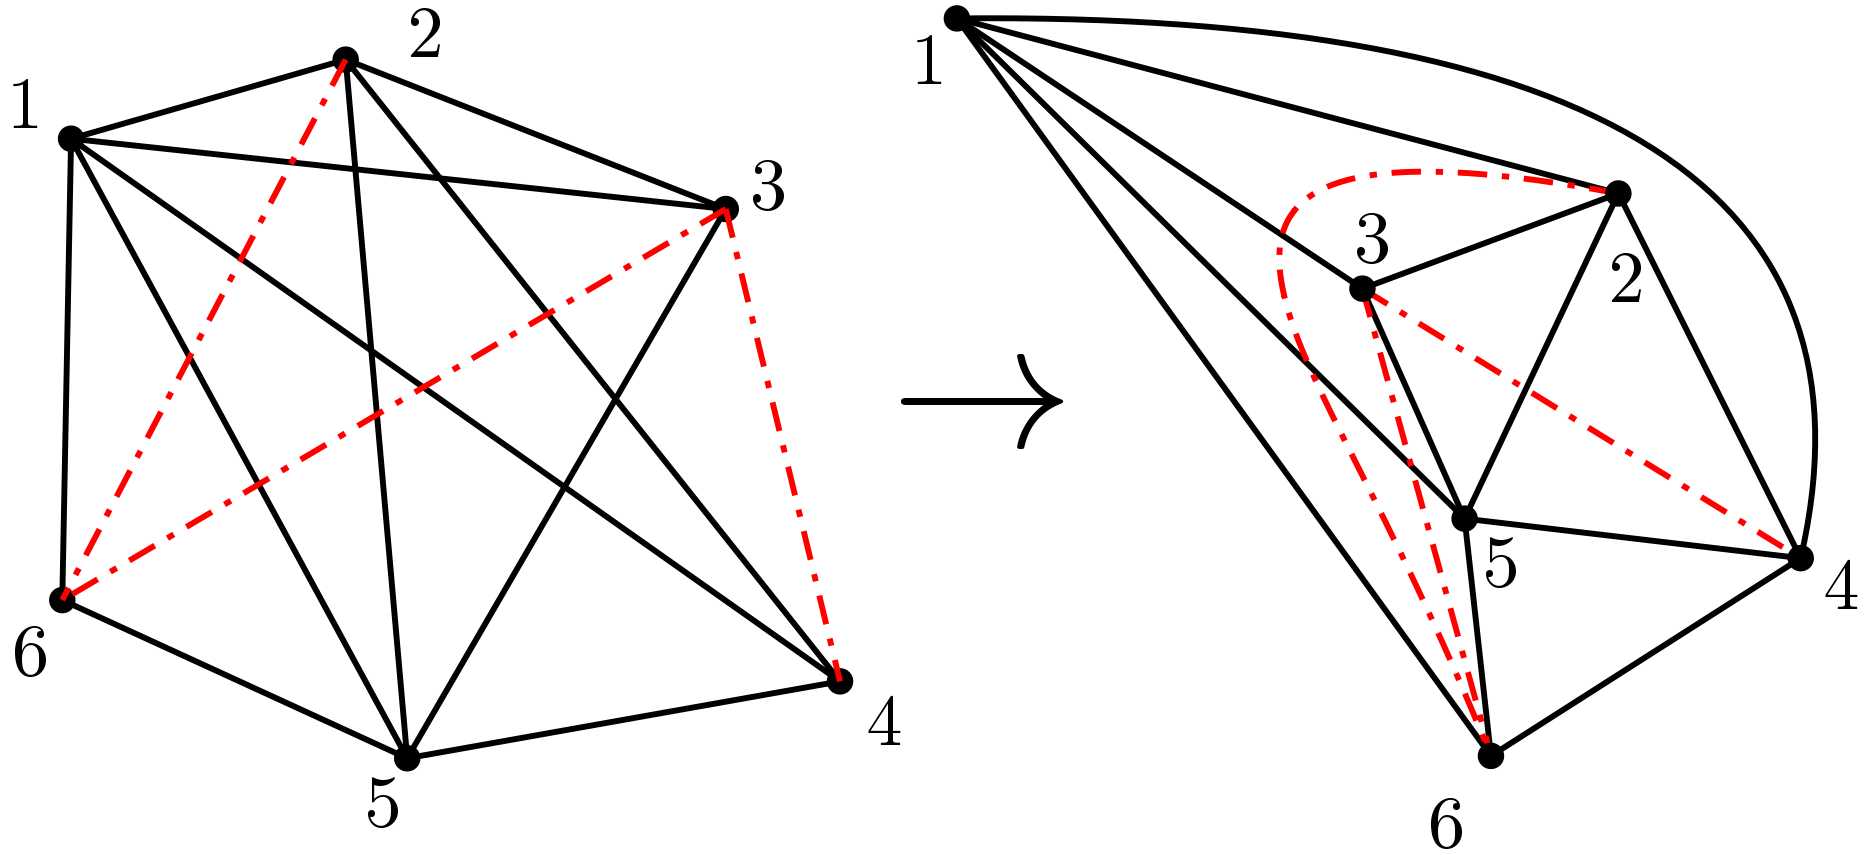
\includegraphics[width=1.4\linewidth]{K6_thicknes2}
  \caption{Una descomposición de tamaño 2 de $K_6$.}
  \label{fig:thk6}
\end{subfigure}%
\\
\begin{subfigure}[h]{.5\textwidth}
  \centering
  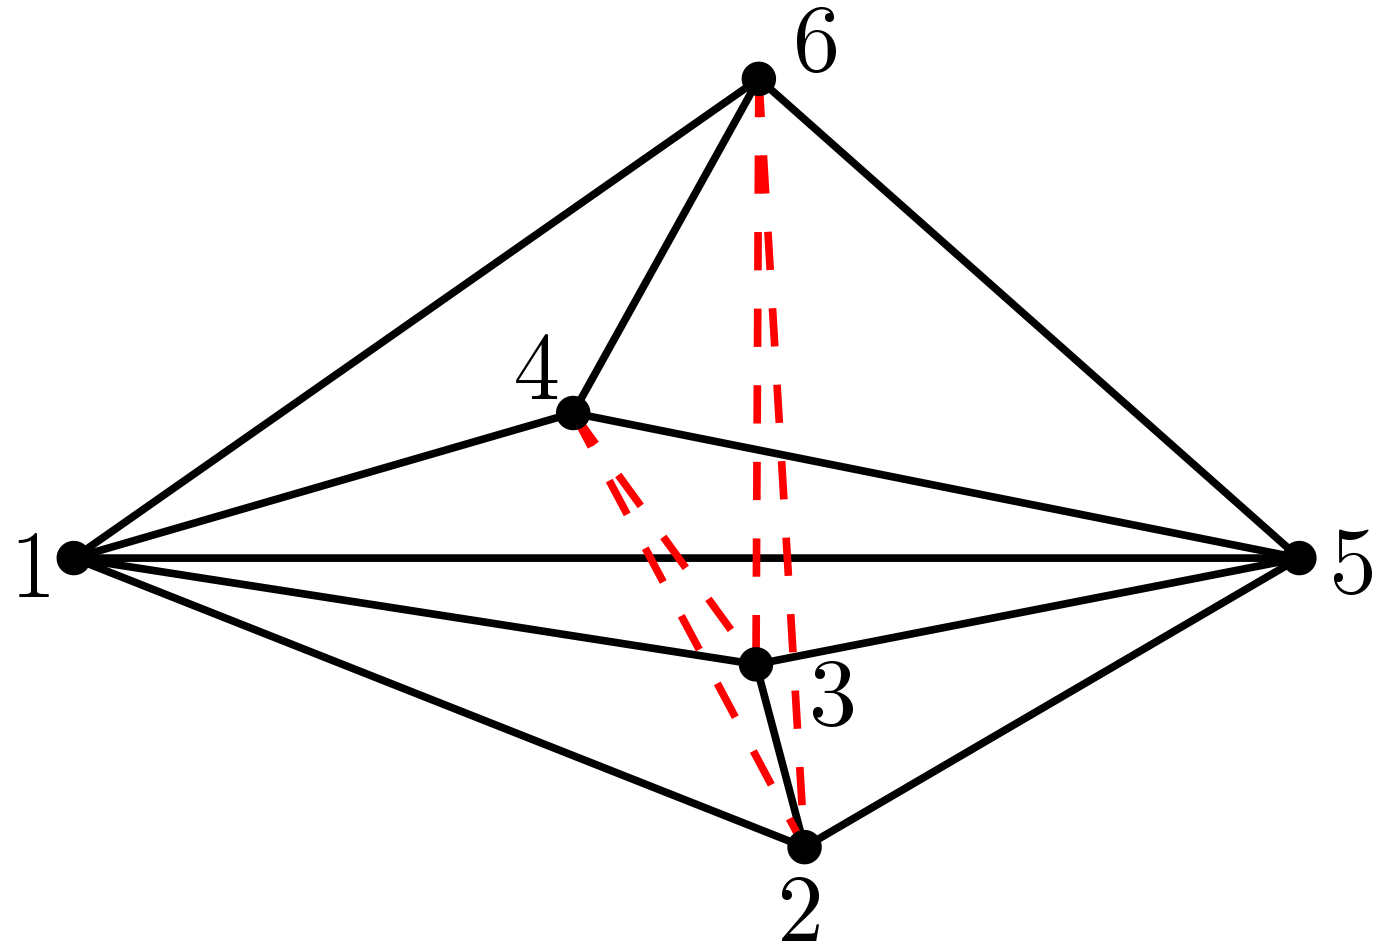
\includegraphics[width=.8\linewidth]{K6_gthicknes2}
  \caption{UN ddibujo geométrico de $K_6$ y su descomposición
  en dos gráficas geométricas planas.}
  \label{fig:gthk6}
\end{subfigure}
\caption{La figura (a) muestra que el thickness de $K_6$ es menor o igual a dos. La figura (b) muestra que el thickness geométrico de $K_6$ es menor o igual a dos.}
\label{fig:thicknessexample}
\end{figure}

% A través de este capítulo nos referimos a la gráfica completa de $n$ vértices
% como $K_n$ ya que los trabajos citados utilizan gráficas completas y además
% es también nuestro objeto de estudio.


% Antes de hablar del anti-thickness y los resultados, es sensato hablar de otro
% concepto llamado \textbf{thickness} pues su definición está estrechamente
% relacionada con el anti-thickness. En el artículo de Eppstein y otros
% \cite{Dillencourt2004} se recupera la definición de thickness teórico y thickness
% geométrico, además proporciona cotas para éste último. Podemos definir el
% thickness de una gráfica en términos del índice cromático de una gráfica y
% mantenerlo coherente con la definición de Eppstein: $\theta(G):$ Mínimo $k$
% tal que existe una partición de las aristas de $G$, de tamaño $k$ en gráficas planares.

% Por otro lado el thickness geométrico $\bar{\theta}(G)$: Mínimo $k$ tal que
% existe un dibujo geométrico $\mathsf{G}$ de $G$ cuyas aristas pueden ser
% particionadas en $k$ gráficas planas.
\cite{Dillencourt2004} demuestran que el thickness geométrico está acotado por:
\[ \left\lceil \frac{n}{5.646} + 0.342 \right\rceil \leq  \bar{\theta}(G) \leq \left\lceil\frac{n}{4}\right\rceil .\]

En el mismo artículo encuentran el valor exacto del thicknes geométrico
de cada gráfica completa con $n$ vértices, para $n\leq 12$, así como para $K_{15}$ y $K_{16}$.
% Para el caso de $n=15$ encuentran el thickness geométrico exacto probando
% que no existen un conjunto de tres triangulaciones del conjunto de puntos que
% cubran las $\binom{15}{2} = 105$ aristas. Para el caso de $n=16$ el resultado
% es exacto usando las cotas dadas.
También estudian el thickness geométrico para gráficas completas bipartitas y demuestran la
siguiente cota:
\[
  \left\lceil \frac{ab}{2a+2b-4} \right\rceil \leq \theta(K_{a,b}) \leq \bar{\theta}(K_{a,b})
  \leq \left\lceil \frac{min(a,b)}{2} \right\rceil.
\]

% A continuación citaremos dos trabajos asociados al anti-thickness cuyo núcleo
% se basa en obtener el número cromático de una gráfica cuyos vértices y aristas
% son abstraidas de una gráfica geométrica definida sobre un conjunto de puntos
% en el plano. Empezaremos por definir la gráfica de cruce $E_{pp}(S)$ de un conjunto
% de puntos $S$ en posición general. Consideremos que existe un dibujo geométrico
% de $K_n$ cuyo conjunto de vértices es $S$.

% A continuación discutimos dos trabajos que están relacionados con el anti-thickness.
% En ambos artículos los autores obtienen el número cromático de una gráfica cuyos vértices
% y aristas abstraen las relaciones de adyacencia de una gráfica geométrica.
Para explicar la relación entre el thickness y el anti-thickness es necesario
hablar de coloraciones de vértices de gráficas de adyacencia. Recordemos que
dadas dos aristas de una gráfica geométrica $\mathsf{G}$, decimos que estas
se intersectan si comparten un vértice o si se cruzan y que son disjuntas
si no se intersectan. La gráfica de adyacencia de una gráfica geométrica
$\mathsf{G}$ tiene como conjunto de vértices a todas las aristas de
$\mathsf{G}$. Dependiendo del tipo de adyacencia que consideremos
podemos definir cuatro diferentes gráficas de adyacencia, estas se listan
a continuación:
\begin{enumerate}
  \item \label{itm:epp}La gráfica de adyacencia en la que existe una arista
  entre dos vértices si las aristas correspondientes en $\mathsf{G}$ se cruzan.
  \item  \label{itm:W} La gráfica de adyacencia en la que existe una arista
  entre dos vértices si las aristas correspondientes en $\mathsf{G}$ comparten
  un vértice o son disjuntas.
  \item  \label{itm:I} La gráfica de adyacencia en la que existe una arista
  entre dos vértices si las aristas correspondientes en $\mathsf{G}$ se
  intersectan.
  \item \label{itm:D}  La gráfica de adyacencia en la que existe una arista
  entre dos vértices si las aristas correspondientes en $\mathsf{G}$ son
  disjuntas.
\end{enumerate}

% \begin{enumerate}
%   \item } Dos aristas se cruzan.
%   \item Dos aristas no se cruzan.
%   \item Dos aristas se cruzan o comparten un vértice.
%   \item Dos aristas son totalmente disjuntas.
% \end{enumerate}
% Dada una gráfica geométrica
% su gráfica de incidencia es construida a partir de las incidencias de aristas de la gráfica geométrica.
Ahora definimos una gráfica a la que llamamos \emph{gráfica de cruce}.

\begin{definition}{\emph{Gráfica de cruce}.}
  Sea $S$ un conjunto de $n$ puntos en posición general en el plano y sea $K_n(S)$ la gráfica completa
  asociada a $S$. La gráfica de cruce $E_{pp}(S)$ de $S$ es la gráfica que tiene un vértice
  por cada arista de $K_n(S)$ y una arista entre dos vértices de $E_{pp}(S)$ si sus aristas correspondientes
  se cruzan en $K_n(S)$.
\end{definition}

La gráfica $E_{pp}(S)$ corresponde a la gráfica de adyacencia \ref{itm:epp}.
\begin{figure}
\begin{subfigure}{.5\textwidth}
  \centering
  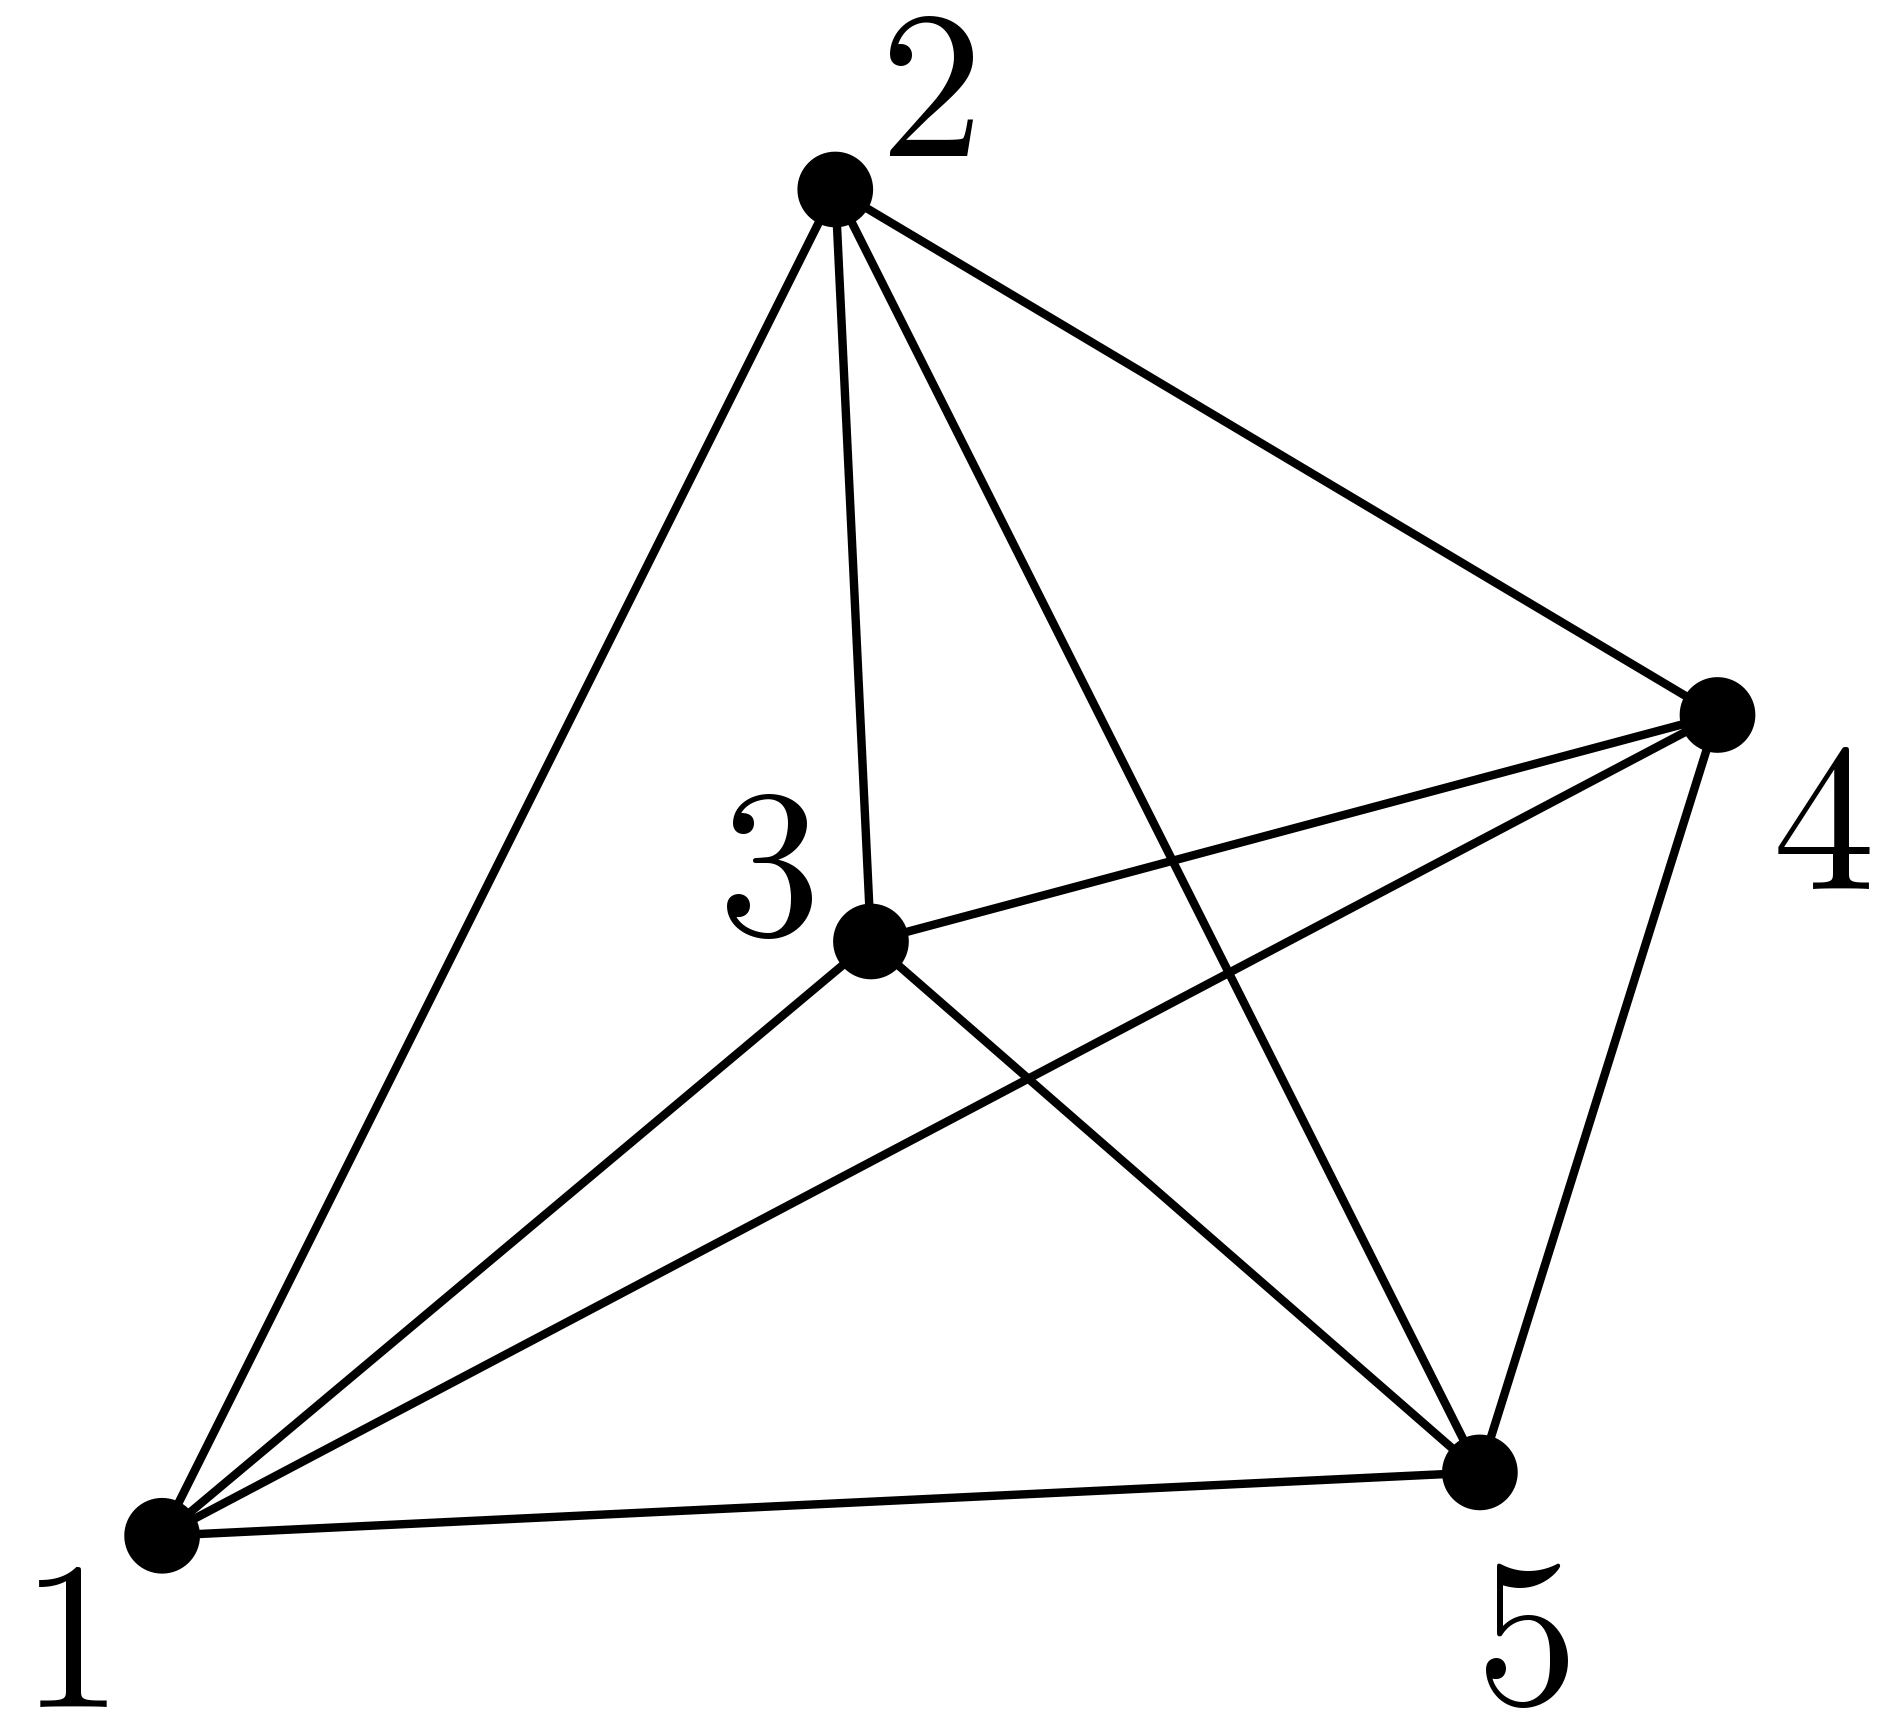
\includegraphics[width=.8\linewidth]{K5}
  \caption{Un dibujo geométrico de $K_5$ cuyo conjunto de vértices es $S=\{1,2,3,4,5\}$.}
  \label{fig:k5}
\end{subfigure}%
\begin{subfigure}{.5\textwidth}
  \centering
  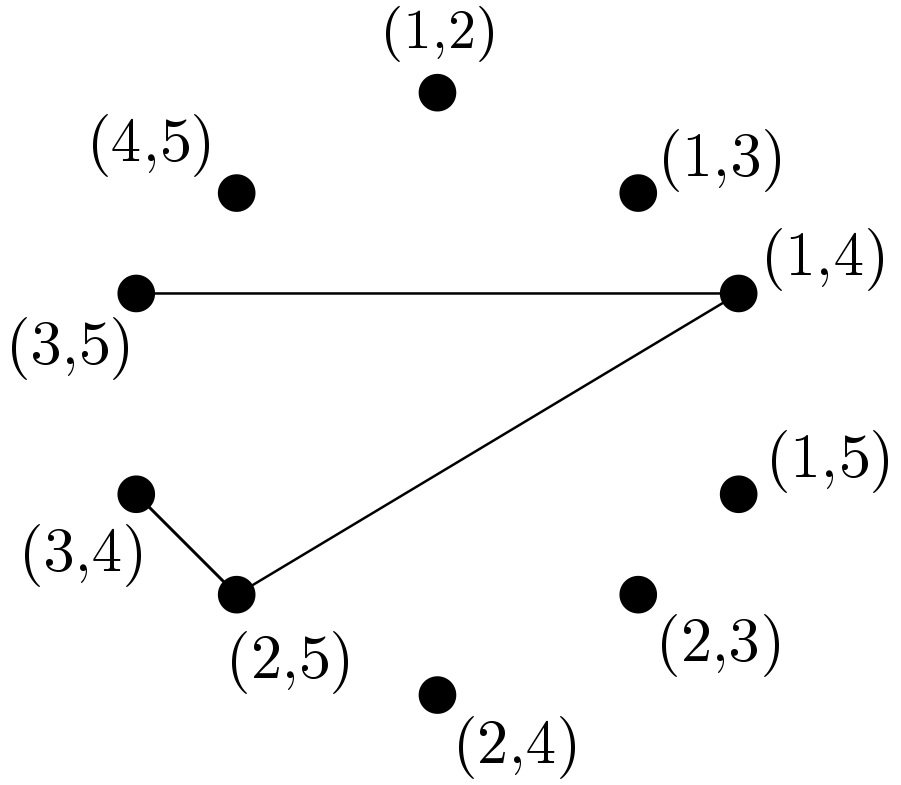
\includegraphics[width=.8\linewidth]{EppK5}
  \caption{La gráfica $E_{pp}(S)$.}
  \label{fig:eppk5}
\end{subfigure}
\caption{Una instancia de $K_5$ y su respectiva gráfica de cruce $E_{pp}(S)$.}
\label{fig:ejemploeppk5}
\end{figure}

En la figura \ref{fig:ejemploeppk5} aparece un ejemplo de la gráfica de cruce $E_{pp}(S)$.
Podemos notar que dado que en el dibujo de $K_5$ hay 3 cruces, en la gráfica $E_{pp}(S)$
hay 3 aristas.
% Los conjuntos independientes de $E_{pp}(S)$ corresponden a conjuntos de aristas
% que las aristas correspondientes en el dibujo de $K_n$ son en efecto gráficas planas.
% Cuando asignamos un color a cada conjunto independiente, tenemos una clase
% cromática por cada conjunto independiente y si minimizamos el número de clases cromáticas
% habremos encontrado una coloración propia de $E_{pp}(S)$ y por consiguiente una descomposición
% en gráficas planas de un dibujo de $K_n$ cuyo tamaño es mínimo, en otras palabras obtenemos
% el thickness de un dibujo en particular de $K_n$.

Los conjuntos independientes de $E_{pp}(S)$ corresponden a conjuntos de aristas de $K_n(S)$
que inducen gráficas planas. Luego, una coloración propia de los vértices de $E_{pp}(S)$
corresponde a una descomposición de $K_n(S)$ en gráficas planas.
Por lo tanto encontrar el número cromático $\chi(E_{pp}(S))$ de la gráfica
$E_{pp}(S)$ es equivalente a encontrar el thickness geométrico de $K_n(S)$.
La figura \ref{fig:k5coloring} ilustra esta relación.
El thickness geométrico de la gráfica completa de $n$ vértices $K_n$ se puede
definir en estos términos como sigue:
\begin{definition}{\emph{Thickness geométrico de una gráfica}.}
  % Considerese $K_n=(S,E)$ la gráfica completa cuyo conjunto de vértices es $S$.
  \[\bar{\theta}(n) = \min\{ \chi(E_{pp}(S)): S \subset \mathbb{R}^2 \text{ está en posición general }, |S|=n \}.\]
\end{definition}
\begin{figure}
  \centering
  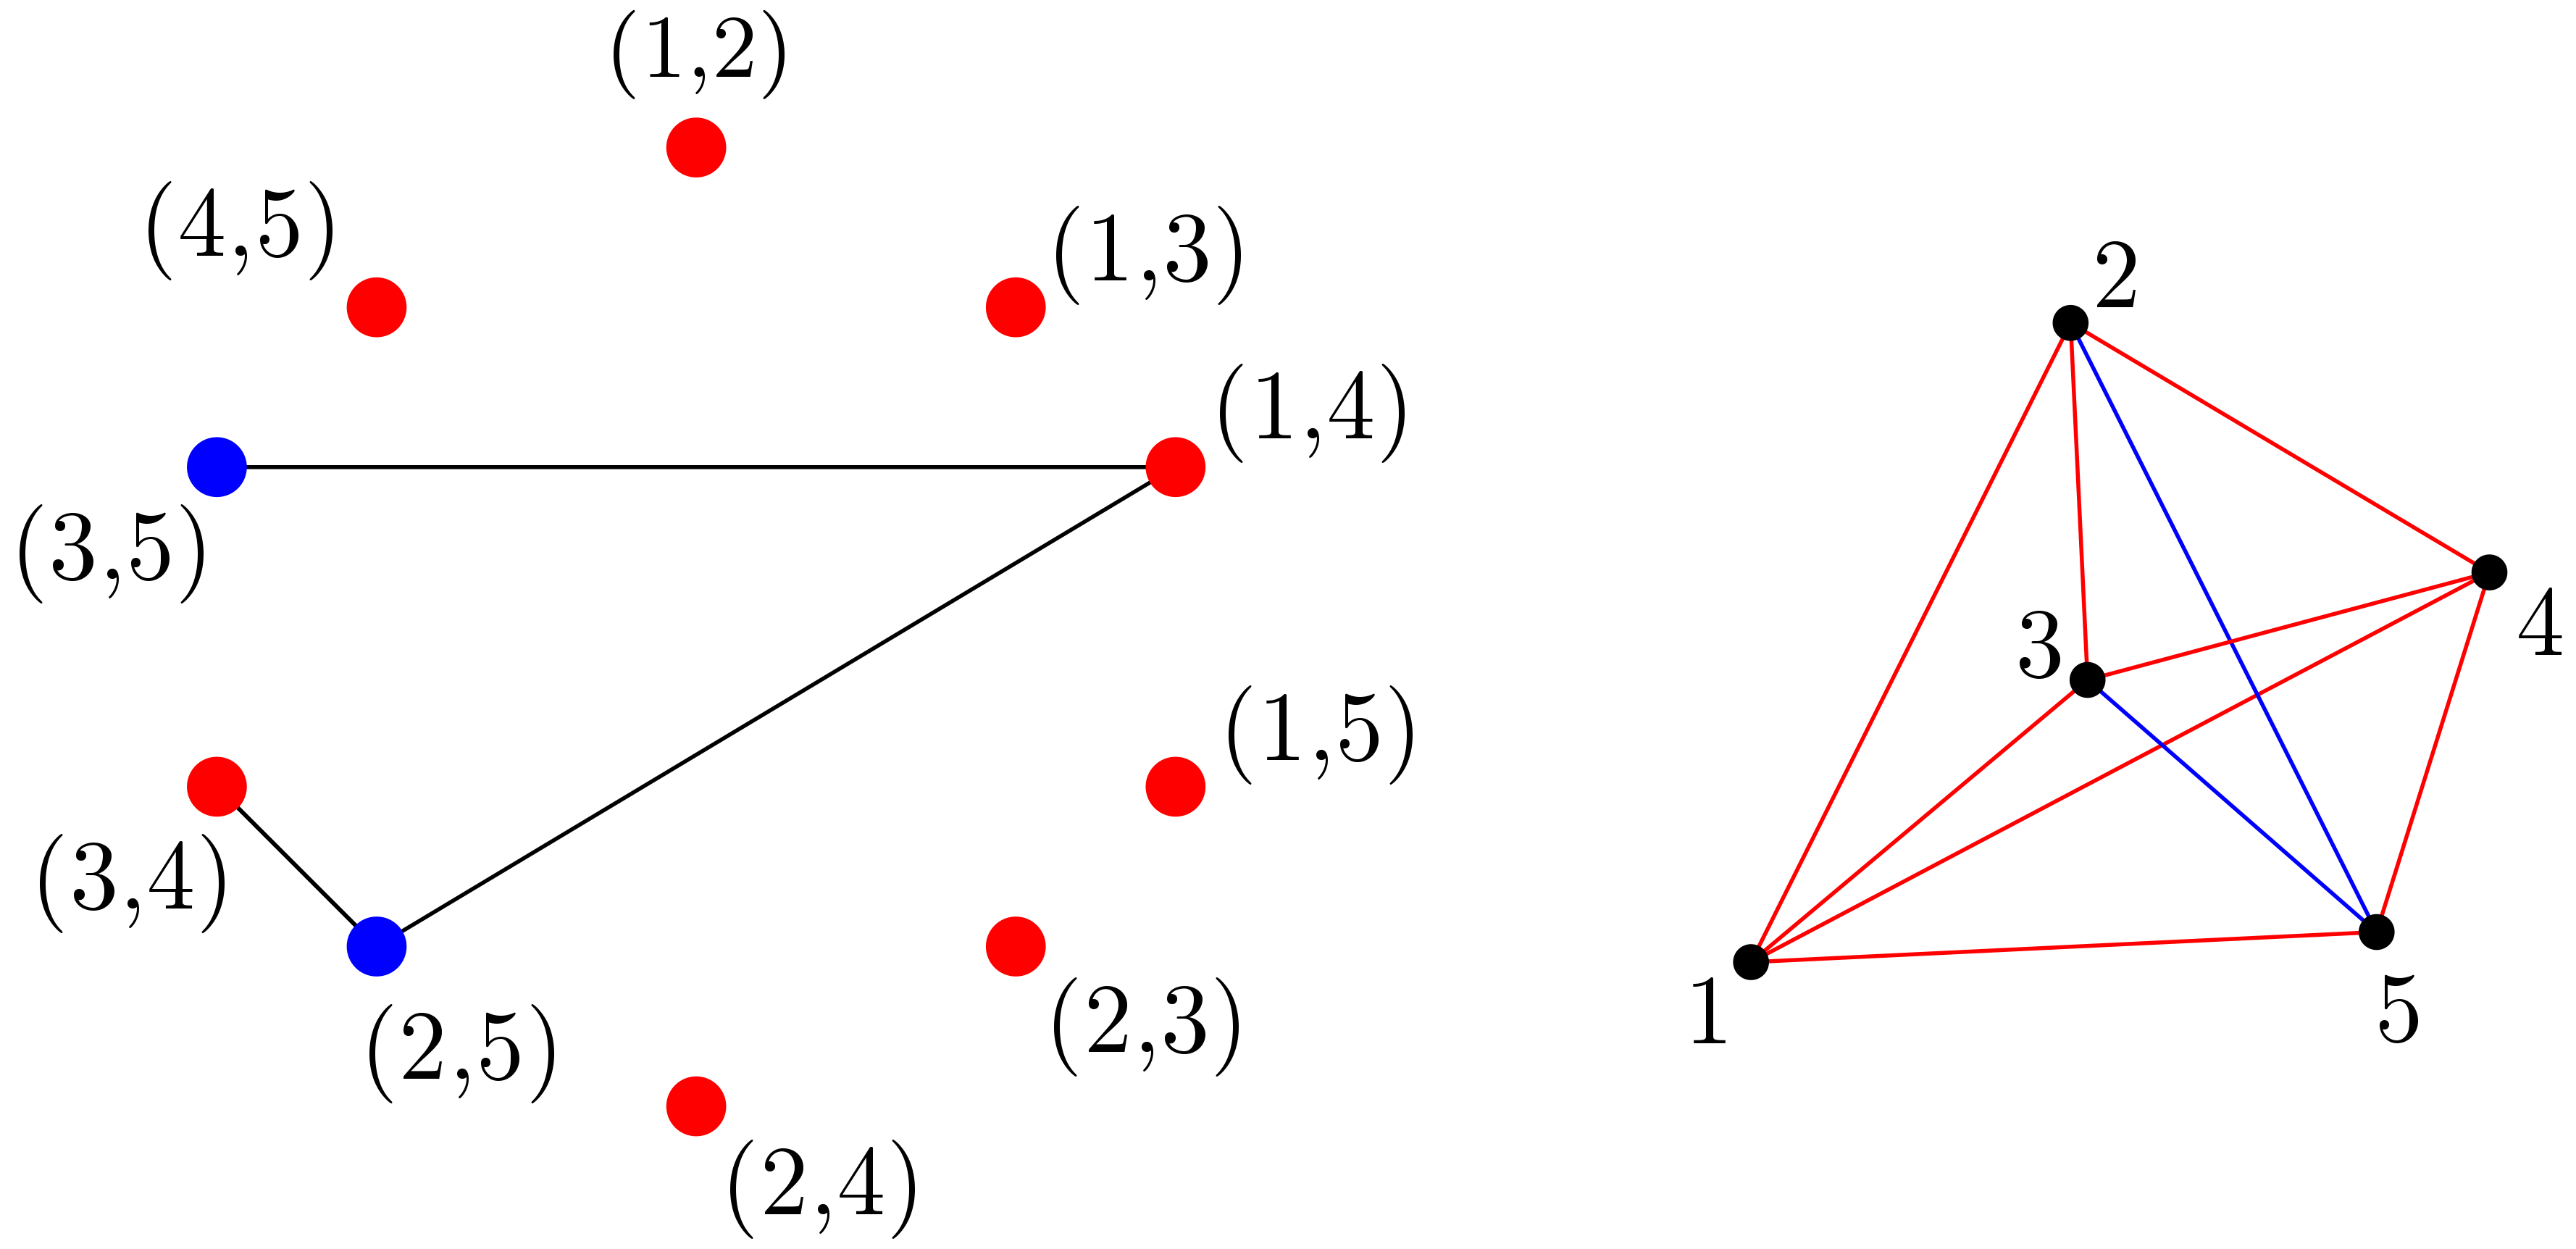
\includegraphics[width=.8\linewidth]{k5coloring}
  \caption{De izquierda a derecha: Una coloración propia de los vértices de $E_{pp}(S)$ con dos
  clases cromáticas indicadas como círculos y cuadros.
  Una descomposición de un dibujo de $K_5$ en dos gráficas planas
  cuyas aristas corresponden a cada una de las clases cromáticas de la coloración
  de $E_{pp}(S)$.}
  \label{fig:k5coloring}
\end{figure}

% \begin{definition}{\emph{Thickness geométrico de un dibujo de una gráfica}.}
%   El thickness geométrico $th_g(G)$ de un dibujo geométrico de $G$ es el número cromático
%   $\chi(E_{pp}(S))$ de la gráfica $E_{pp}(S)$ donde $S$ es el conjunto de vértices de $K_n$.
% \end{definition}

% \begin{definition}{\emph{Thickness geométrico de una gráfica geométrica}.}
% Sea $\mathsf{G}$ una gráfica geométrica completa definida sobre un conjunto de puntos $S$,
% el thickness geométrico $th(\mathsf{G})$ de $\mathsf{G}$ es el número cromático
% $\chi(E_{pp}(S))$ de la gráfica $E_{pp}(S)$.
% \end{definition}

% Y luego, siguiendo la definición de \cite{Dillencourt2004} redefinimos el thickness
% geométrico de la gráfica completa de $n$ vértices $K_n$, como el thickness geométrico
% más pequeño de de todos los dibujos posibles de la gráfica.
% A este número le llamaremos $epp(n)$ y lo definimos formalmente como:

%
% De la misma manera que definimos la gráfica de cruce $E_{pp}(S)$ podemos definir
% otras gráficas si cambiamos la condición bajo la cual existen aristas entre vértices
% de $E_{pp}(S)$. En este sentido, en el trabajo de \cite{Araujo2005}, se definen
% varias gráficas que se listan en seguida. Para todas existe una gráfica geométrica
% completa $K_n$ cuyo conjunto de vértices es $S$.

De la misma manera que definimos la gráfica de cruce podemos definir otras
gráficas de adyacencia. Para esto basta con considerar alguno de los otros
tipos de adyacencia. En este sentido, en el trabajo de~\cite{Araujo2005} se
definen las gráficas que se listan en seguida, cada una corresponde
a una de las cuatro gráficas de adyacencia mencionadas anteriormente.
Sea $S$ un conjunto de $n$ puntos en posición general y $K_n(S)$
la gráfica completa asociada a $S$:

% Sea $S$ un conjunto de puntos en posición general con $|S|=n$ y sea $K_n(S)$ la gráfica completa
% asociada a $S$. La gráfica de cruce $E_{pp}(S)$ de $S$ es la gráfica que tiene un vértice
% por cada arista de $K_n(S)$ y una arista entre dos vértices de $E_{pp}(S)$ por cada par de aristas
% que se crucen en $K_n(S)$.
\begin{itemize}
  \item $W(S):$ Es la gráfica correspondiente a la gráfica de adyacencia
  \ref{itm:W}.
  \item $I(S):$ Es la gráfica correspondiente a la gráfica de adyacencia
  \ref{itm:I}.
  \item $D(S)$  Es la gráfica correspondiente a la gráfica de adyacencia
  \ref{itm:D}.
\end{itemize}
A partir de aquí, nos referimos a las gráficas de adyacencia 1,2,3 y 4 como
$E_{pp}(S),W(S),I(S)$ y $D(S)$ respectivamente.
% \begin{itemize}
%   \item $W(S):$ Es la gráfica que tiene un vértice por cada arista de $K_n(S)$ y
%   una arista entre dos vértices de $W(S)$ si sus aristas correspondientes en $K_n(S)$
%   cumplen con el criterio \ref{itm:W}.
%   \item $I(S):$ Es la gráfica que tiene un vértice por cada arista de $K_n(S)$ y
%   una arista entre dos vértices de $I(S)$ si sus aristas correspondientes en $K_n(S)$
%   cumplen con el criterio \ref{itm:I}.
%   \item $D(S)$ Es la gráfica que tiene un vértice por cada arista de $K_n(S)$ y
%   una arista entre dos vértices de $D(S)$ si sus aristas correspondientes en $K_n(S)$
%   cumplen con el criterio \ref{itm:D}.
% \end{itemize}

Es fácil darse cuenta que la condición de existencia de aristas de $W(S)$ es
complementaria a la condición en $E_{pp}(S)$ y viceversa. De la misma
forma, las condiciones de $I(S)$ y $D(S)$ son complementarias entre sí. En la tabla~\ref{table:graficasincidencia}
mostramos esta relación y las estructuras geométricas
que representan, en $K_n(S)$, los conjuntos independientes para cada gráfica de adyacencia.

\emph{Open problem garden} es un sitio web en el que investigadores de diferentes áreas
de las matemáticas como algebra, combinatoria, teoría de números o teoría de gráficas
publican problemas abiertos para que la comunidad pueda leerlos libremente.
En este sitio web~\cite{OpenGarden2009} presenta un problema en el que se requiere asignar un
color a cada arista de una gráfica geométrica completa bajo cada una de los cuatro
criterios de adyacencia mencionados antes.

% En el aporte de \cite{Araujo2005} buscan el número cromático de cada una de las
% gráficas listadas anteriormente por lo que creemos sensato decir a qué estructuras
% geométricas en el dibujo de $K_n$ equivale una clase cromática de cada alternativa.
% Para $W(S)$ una clase cromática equivale a un emparejamiento de cruce (\emph{crossing matching}),
% para $I(S)$ equivale a un emparejamiento sin cruce (\emph{non-crossing matching})
% y para $D(S)$ equivale a un thrackle.
%
% El hecho de que la coloración de $D(S)$ otorgue una descomposición en thrackles es la
% principal razón por la cual el trabajo es de importancia para nosotros. Sin embargo,
% en \cite{Araujo2005} se busca el máximo número cromático para cada dibujo posible
% de $K_n$ para cada una de las tres gráficas listadas anteriormente. Concretamente
% ellos definen los siguiente:
\begin{table}
  \centering
  \begin{tabular}{|l|l|}
    \hline
    Gráfica   & Conjuntos independientes en $K_n(S)$    \\ \hline \hline
    $W(S)$    & \emph{Emparejamientos de cruces}        \\ \hline
    $I(S)$    & \emph{Emparejamientos planos}           \\ \hline
    $D(S)$    & \emph{Thrackles}                        \\ \hline
    $E_pp(S)$ & \emph{Gráfica planar}                   \\ \hline
  \end{tabular}
  \caption{Esta tabla muestra qué representan los conjuntos independientes en $K_n(S)$
  para cada una de las gráficas definidas en \cite{Araujo2005} y para $E_pp(S)$.}
  \label{table:graficasincidencia}
\end{table}
En el artículo de \cite{Araujo2005} buscan el número cromático de cada una de las
gráficas de adyacencia mencionadas anteriormente, los autores estudian los siguientes parámetros:
  \begin{align*}
    w(n) &= \max\{\chi(W(S)): S\subset \mathbb{R}^2 \text{ está en posición general}, |S|=n\}. \\
    i(n) &= \max\{\chi(I(S)): S\subset \mathbb{R}^2 \text{ está en posición general}, |S|=n\}. \\
    d(n) &= \max\{\chi(D(S)): S\subset \mathbb{R}^2 \text{ está en posición general}, |S|=n\}. \\
  \end{align*}
% Para cada uno también definen el caso en el que $S \subset \mathbb{R}^2$ está
% en posición convexa como $w_c(n)$, $i_c(n)$ y $d_c(n)$ y demuestran las siguientes cotas:
Para el caso en el que $S$ está en posición convexa se denotan a estos valores como
$w_c(n)$, $i_c(n)$ y $d_c(n)$. Los autores demuestran las siguientes cotas:
\begin{itemize}
  \item $w_c(n) = \Theta(n\log n)$.
  \item $c_1n\log n \leq w(n) \leq c_2 n^2 \frac{\log\log n}{\log n}, \text{ para } c_1,c_2 > 0$.
  \item $i_c(n) = n$.
  \item $n \leq i(n) \leq Cn^{3/2} \text{ para } C > 0$.
  \item $2\lfloor \frac{n+1}{3}\rfloor -1 \leq d_c(n) \leq \min\left( n-2, n - \frac{\lfloor{\log n}\rfloor}{2}\right)$.
  \item $5\lfloor \frac{n}{7}\rfloor \leq d(n) \leq \min\left(n-2,n+\frac{1}{2}- \frac{\lfloor{\log \log n}\rfloor}{n}\right)$.
\end{itemize}

A pesar de que en el trabajo de~\cite{Araujo2005} se busca el número cromático
de la gráfica $D(S)$ y con ello, de manera implicita, buscar el anti-thickness de una gráfica
geométrica asociada a $S$, es importante notar que la definición $d(n)$ no es
equivalente a la de anti-thickness. Dada una gráfica $G$: en $d(n)$ se busca el máximo de todos los
números cromáticos para todas las gráficas geométricas de $G$
mientras que en el anti-thickness se busca el mínimo de todos los números cromáticos para todas
las gráficas geométricas de $G$.

Podemos dar una definición del anti-thickness geométrico usando la gráfica $D(S)$
como sigue:
\begin{definition}{\emph{Anti-thickness geométrico de una gráfica}.}
  \[At_g(n) = \min\{\chi(D(S)): S\subset \mathbb{R}^2 \text{ está en posición general}, |S|=n\}.\]
\end{definition}

De manera análoga si los puntos de $S$ están en posición convexa definimos el
anti-thickness convexo:

\begin{definition}{\emph{Anti-thickness convexo de una gráfica}.}
  \[At_c(n) = \min\{\chi(D(S)): S\subset \mathbb{R}^2 \text{ está en posición convexa}, |S|=n\}.\]
\end{definition}

El anti-thickness convexo de la gráfica completa de $n$ vértices es equivalente
a $d_c(n)$.
% Por otro lado, debido a que cuando $K_n$ es dibujado en el plano en posición convexa
% los dibujos posibles no presentan diferencias combinatorias se tiene que el
% anti-thickness convexo de la gráfica completa de $n$ vértices es equivalente a la definición
% de $d_c(n)$ de \cite{Araujo2005}, dicho de otra forma:
% \[ d_c(n) = cat(n)\]
% Es natural pensar que si una gráfica puede ser descompuesta en sub-gráficas donde
% no existe ningún cruce entre dos aristas, es quizás posible descomponer la
% gráfica en sub-gráficas donde siempre ocurran cruces entre dos aristas, es decir
% en thrackles; este concepto es conocido como el anti-thickness de una gráfica y
% analogo al caso del thickness también existe el anti-thickness geométrico.

% Antes de examinar los resultados del anti-thickness, resulta interesante verificar
% el trabajo de Araujo y Urrutia \cite{Araujo2005}; aquí se define la gráfica de
% disyunción $D(S)$ de un conjunto $S$ de puntos en el plano, donde considerando
% todos los segmentos de recta entre pares de vértices de $S$ como los vértices
% de $D(S)$, existe una arista entre dos vértices si los dos segmentos
% de recta correspondientes se cruzan o comparten un vértice.

% Si asignamos un color a cada vértice de $D(S)$ de tal manera que dos
% vértices adyacentes no compartan color y además minimizamos el número de colores
% usados, obtenemos el número cromático de $\chi(D(S))$. Es fácil ver que una
% clase cromática de $D(S)$ es un conjunto independiente y además un thrackle. Si
% ahora consideramos todos los posibles encajes de $S$ en el plano y para cada uno
% encontramos $\chi(D(S))$, tendremos una lista de enteros que representa el tamaño
% mínimo de la descomposición en thrackles de una gráfica completa cuyos
% vértices están dados por $S$ en el plano. Si de esta lista consideramos ahora
% el valor mínimo encontraremos el anti-thickness para la gráfica completa geométrica de
% $n$ vértices. Sin embargo, en este trabajo se considera el máximo valor de dicha lista;
% definiendo entonces :
% \[ d(n) = \max\{\chi(D(S)): S \subset \mathbf{R}^2 \text{ en posición general }, |S|=n\}\]
%
% De manera concreta, el trabajo presenta cotas para $d(n)$, y $d_c(n)$ que se define
% de manera similar pero con $S$ en posición convexa.
%
% La diferencia entre $d(n)$ y el anti-thickness reside en que el último buscamos el
% mínimo de la lista de números cromáticos de $D(S)$, para ver más claramente
% la relación entre $d(n)$ y el anti-thickness podemos definir el
% anti-thickness geométrico de la gráfica completa de n vértices $at(n)$ como sigue :
% \[ at(n) = \min\{\chi(D(S)): S \subset \mathbf{R}^2 \text{ en posición general }, |S|=n\}\]

%
% Como se mencionó anteriormente el anti-thickness está relacionado con la descomposición
% de una gráfica en sub-gráficas donde siempre ocurren cruces, podemos ver el
% anti-thickness como el lado opuesto del thickness.
Los autores de \cite{Dujmovic2017} presentan resultados respecto a el
anti-thickness para familias específicas de gráficas como árboles, gráficas
outerplanar, y algunos dibujos como 2-tracks, books, k-queues, entre otros.

En su trabajo definen en anti-thickness como sigue:
\begin{definition}{\emph{Anti-thickness de una gráfica.}}
Sea $G$ una gráfica el anti-thickness $At(G)$ de $G$ es el mínimo entero $k$
para el cual existe una partición de $E(G)$ de tamaño $k$
en la que cada elemento de la partición induce una gráfica thrackleable.
\end{definition}

Además dan una relación entre el thickness y anti-thickness de cualquier
gráfica. Concretamente los autores prueban la siguiente cota para toda gráfica
con anti-thickness $k$ y thickness $t$:
\[ k \leq t \leq \left\lceil \frac{3k}{2}\right\rceil .\]

Acerca del anti-thickness de gráficas completas, en el mismo artículo
prueban que \[ \frac{n}{3} \leq  At(K_n) \leq \left\lceil \frac{n-1}{2} \right\rceil . \]

Ellos conjeturan que el anti-thickness de una gráfica completa es
exactamente $\left\lceil \frac{n-1}{2} \right\rceil$.
% Los resultados presentados en ese trabajo que tienen que ver con el anti-thickness
% geométrico de una gráfica completa se enfocan  en el caso específico de puntos en posición convexa.

En los siguientes párrafos describimos cómo los autores de~\cite{Fabila-Monroy2018}
encuentran el anti-thickness geométrico exacto para gráficas cuyo conjunto
de vértices está en posición convexa.

Los autores prueban que bajo esta condición dos thrackles máximos siempre
comparten al menos una arista. Por lo anterior la unión de $k$ thrackles máximos tiene
a lo sumo $kn - \binom{k}{2}$ aristas. Entonces, como una gráfica completa de $n$
vértices tiene $\binom{n}{2}$ aristas la resolución de la desigualdad
\[ \binom{n}{2} \leq kn - \binom{k}{2} .\]
otorga el resultado de la cota inferior para el anti-thickness convexo. Esta cota es:
\[ At_c(K_n) \geq n - \Bigl\lfloor \sqrt{2n + \frac{1}{4}} - \frac{1}{2} \Bigr\rfloor. \]

La cota superior se obtiene dando una coloración propia de los vértices de la gráfica
$D(S)$. Recordemos que una coloración propia de $D(S)$ equivale a encontrar el
antithickness de la gráfica completa asociada a $S$.
En el articulo logran la coloración trazando caminos en una
estructura conocida como poliominó~\cite{Fabila-Monroy2018-poly}
en la que los vértices de $D(S)$ son las filas y las columnas de dicha estructura.
En dicho trabajo cada camino representa un conjunto independiente de vértices en
 $D(S)$ y por lo tanto, respresenta un thrackle en $K_n$.
Los autores concluyen dando el número máximo de caminos posibles en el
polyomino, dicho número coincide con el de la cota inferior y luego se tiene
que el anti-thickness convexo tiene exactamente el siguiente valor:
\[ At_c(n) = n - \Bigl\lfloor \sqrt{2n + \frac{1}{4}} - \frac{1}{2} \Bigr\rfloor \]

A continuación hablamos del trabajo de~\cite{Lomeli2018} en donde encuentran el
anti-thickness geométrico de la doble cadena convexa. La doble cadena convexa
es una configuración de puntos conformada por una $k\text{-}cup$ y una
$l\text{-}cap$. La $k\text{-}cup$ es una cadena de $k$ puntos en posición
convexa donde la parte superior de su cubierta está delimitada por un solo
segmento. La $l\text{-}cap$ es una cadena de $l$ puntos en posición convexa
donde la parte inferior de su cubierta está delimitada por un solo segmento. En
el artículo la doble cadena convexa $C_{k,l}$ que definen tiene las siguientes
características:
\begin{itemize}
  \item Para $l\geq k$ la doble cadena convexa es la unión una $k\text{-}cup$ $U$ y una $l\text{-}cap$ $L$.
  \item Cada punto de $L$ está por debajo de cada segmento de recta definido por dos puntos de $U$.
  \item Cada punto de $U$ está por arriba de cada segmento de recta definido por dos puntos de $L$.
\end{itemize}

La figura \ref{fig:exdoblecadena} muestra un ejemplo de una doble cadena
convexa.
\begin{figure}[htpb]
  \centering
  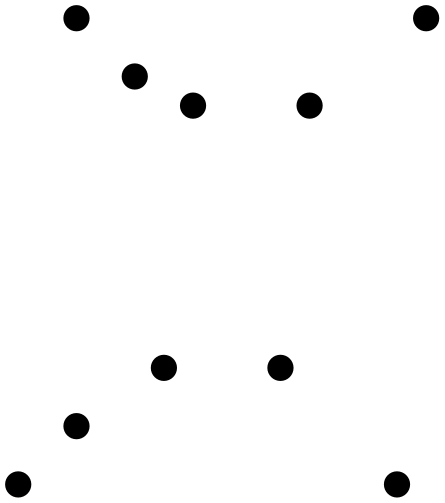
\includegraphics[width=0.2\linewidth]{exdoblecadena}
  \caption{Una doble cadena convexa con 5 vértices en su $k\text{-}cup$ y 5 vértices en su $l\text{-}cap$.}
  \label{fig:exdoblecadena}
\end{figure}

El resultado al que se llega en ese trabajo es que el anti-thickness geométrico
de la doble cadena convexa con $k$ puntos en la cadena convexa superior
y $l$ puntos en la cadea convexa inferior es:
 \[At_g(K_{l,k}) = k+l-\Bigl\lfloor \sqrt{2l+\frac{1}{4}} - \frac{1}{2} \Bigr\rfloor\]

 ~\cite{Dujmovic2017} mencionan que encontrar el anti-thickness geométrico de
 gráficas completas en posición general es un problema abierto. En esta tesis
 abordamos este problema para $n\leq 10$.

 Hasta ahora las mejores cotas conocidas para el anti-thickness geométrico son :
 \[\Bigl\lfloor\frac{n-1}{2}\Bigr\rfloor \leq At_g(K_n) \leq n - \Bigl\lfloor
 \sqrt{2n + \frac{1}{4}} - \frac{1}{2} \Bigr\rfloor \]
 La cota superior se sigue del caso convexo y la cota inferior
 se sigue del hecho de que una gráfica de $n$ vértices
 con anti-thickness geométrico $k$ tiene a lo sumo $kn$ aristas.

Los trabajos mencionados en este capítulo muestran cómo el problema original del
thickness está relacionado con problema del anti-thickness. Mostramos de qué
manera un problema de descomposición de gráficas geométricas equivale
a un problema de coloración de gráficas. Los artículos más recientes tratan al
anti-thickness como un problema de coloración. En este trabajo no construimos la
gráfica $D(S)$ y no coloreamos ninguna gráfica. Nuestro enfoque es geométrico
y computacional.

% Es importante notar que el anti-thickness convexo es acotado examinando el número mínimo
% y máximo de aristas aportadas por una colección de thrackles máximos, dicho de
% otra manera se basa en descomponer la gráfica completa convexa en thrackles máximos.
% Esta idea fue retomada en este trabajo para intentar ajustar las cotas del anti-thickness
% en posición general.

Es importante notar que en el trabajo de~\cite{Fabila-Monroy2018} las descomposiciones
de la gráfica completa están conformadas por thrackles máximos. Esta es una de las ideas que
usamos en este trabajo para intentar ajustar las cotas del anti-thickness en posición
general.
